\documentclass[12pt,onecolumn,letterpaper]{article}

\usepackage{xeCJK}
\usepackage{indentfirst}
\usepackage{graphicx}
\usepackage{cite}
\usepackage{amsmath}
\usepackage{amssymb}

\setCJKmainfont{Noto Sans Mono CJK SC}
\setCJKsansfont{Noto Sans Mono CJK SC}
\setCJKmonofont{Noto Sans Mono CJK SC}
\linespread{1.5}
\setlength{\parindent}{2em}


\begin{document}
    \title{人工神经网络原理期末书籍阅读学习报告作业}
    \author{17363092 叶茂青}

    \maketitle

    \section{神经网络控制系统}
    人工神经网络是由大量处理单元连接而成的网络,由于人工神经网络对于任意函数的逼近能力,人工神经网络也被应用于建模困难的非线性控制系统中。
    相比传统控制系统,基于神经网络的控制系统有以下特点:
    \begin{itemize}
        \item 对非线性系统的优良拟合能力
        \item 对并行处理友好
        \item 优秀的学习和自适应能力
        \item 适用于多变量系统
    \end{itemize}


    \section{神经网络控制模型}
    控制系统的模型可分为前向模型和逆模型,在基于神经网络的控制系统中,前向模型的建立如Fig 1,用被控对象输出和神经网络输出的误差训练神经网络,也可以引入RNN网络的结构,将之前模型的信息引入进模型的训练中。
    \begin{figure}[htb]
        \centering
        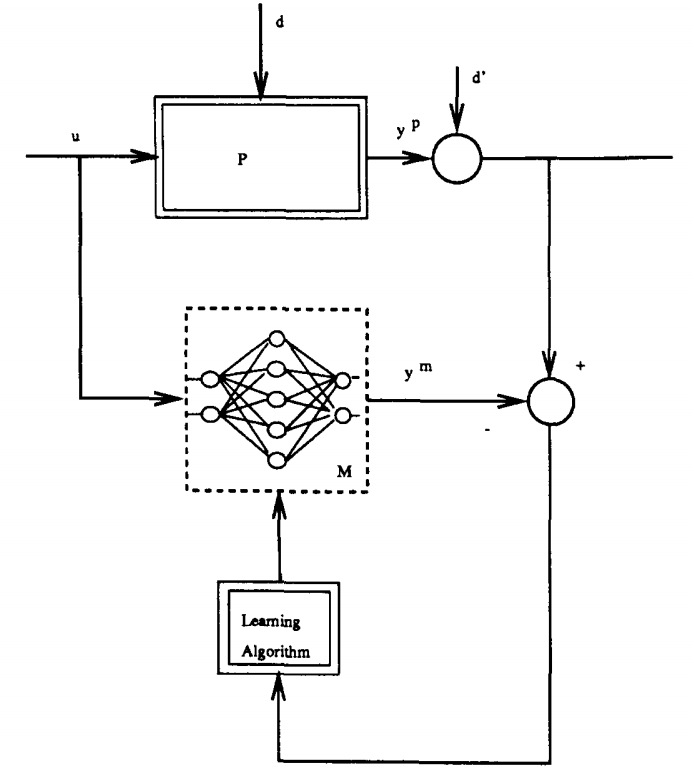
\includegraphics[width=\linewidth]{figure/forward.png}
        \caption{Forward model structures\cite{hunt1992neural}}
    \end{figure}

    逆模型的建立如Fig 2,Direct method中直接将被控对象的输入输出作为神经网络的训练样本,Specialized method则使用两个神经网络建立逆模型,将前向神经网络模型与被控对象并联,逆模型接受被控对象或前向神经网络模型或两者的结合作为训练样本,减弱对真实模型的依赖,且避开了Direct method中要求被控对象的输入输出映射是可逆映射的问题。
    \begin{figure}[htb]
        \centering
        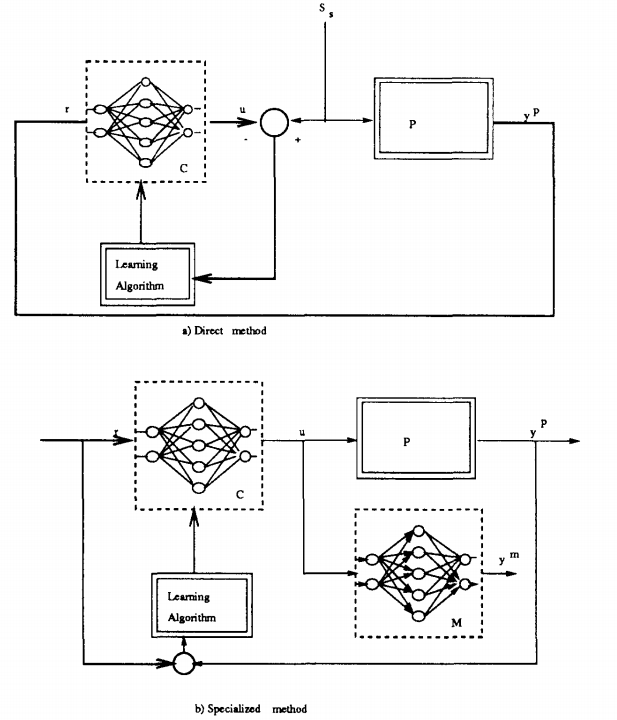
\includegraphics[width=\linewidth]{figure/inverse.png}
        \caption{Inverse model structures\cite{hunt1992neural}}
    \end{figure}

    \subsection{神经网络控制结构}
    Hunt et al.\cite{hunt1992neural}总结了几种常见的神经网络控制结构:
    \begin{itemize}
        \item Supervised control.此类模型的神经网络依靠人工生成的输入输出数据进行学习。典型的例子是Grant et al.\cite{grant1989neural}利用该模型解决pole-cart control的问题。
        \item Direct inverse control.此类模型与之前提到的Direct method类似,神经网络的输入是被控对象的输出,通过让神经网络还原被控对象的输入建立逆模型。此类模型在机器人控制领域中十分常见。
        \item Model reference control.在此类模型中,神经网络的输出与一个参考模型做对比,神经网络的目标是最小化与参考模型输出的误差。
        \item Internal Model Control.此类模型的结构与之前提到的逆模型建模中使用的Specialized method类似,不过会加入滤波器以提高模型的鲁棒性。Hunt et al.\cite{hunt1991neural}实现了用于非线性系统的Internal Model Control.
        \item Predictive control.在此类模型中,神经网络学习的目标是预测被控对象未来一段时间的输出。Keerthi et al.\cite{keerthi1986moving}和Mayne et al.\cite{mayne1988receding}均证明了该方法在非线性系统中具有理想的稳定性。
    \end{itemize}



    \section{神经网络控制的实际应用}
    在神经网络模型的选择上,由于RBF网络相比BP网络的学习速度更快,且可以避免局部极小的问题,在控制系统中,普遍使用RBF网络作为神经网络的模型,以满足对于在线学习的需求。

    神经网络在控制系统的应用主要有两种方式,一是使用神经网络与传统的控制方法(如PID控制器,滑膜控制)相结合,相关的研究有Shu et al.\cite{shu2000pid}提出的可用于时滞系统的PIDNN,Chen et al.\cite{chen2004applying}提出在非线性系统中,使用神经网络调节PID控制器参数的通用模型,并提出动量滤波器,设定更新准则等方法以改善模型的表现,Wang et al.\cite{wang2009neural}利用RBF神经网络建立机械手的动力学模型,并结合滑膜控制用于系统控制,还有Bose et al.\cite{bose2007neural}提出的在电机驱动中,利用神经网络进行滤波,自适应磁通量估计,两级和多级逆变器的PWM等。这类方法在传统控制方法上进行改进,使用神经网络建模复杂的非线性系统,再通过传统的控制方法进行控制,在保证系统稳定性的同时也提升了控制系统的表现。

    二是直接用神经网络作为控制器,如Sanner et al.\cite{sanner1991gaussian}提出的基于RBF网络的直接自适应控制方法,Sutton et al.\cite{sutton1992reinforcement}利用Q-learning算法进行直接自适应控制,Vamvoudakis et al.\cite{vamvoudakis2010online}使用actor-critic算法训练模型。直接使用神经网络作为控制器免去了很多繁琐的建模过程,这类方法普遍也采用model-free的强化学习方法。


    \section{未来方向}
    神经网络控制系统在许多控制问题上均表现出良好的结果,但要让神经网络广泛应用于控制系统依然有很多问题需要解决,这里提出几个方面:
    \begin{itemize}
        \item 如何选取合适的神经网络模型和神经网络控制结构?尽管神经网络在许多问题上表现出了出色的学习能力,但如何选择模型,训练模型,对于网络层数、隐层结点个数、学习率等超参数的设定依然需要繁杂的实验,缺乏理论上的指导。
        \item 如何保证神经网络的鲁棒性?对于控制系统而言,稳定性是十分重要的,所以大部分研究并没有直接使用神经网络作为控制器,而是结合传统的控制方法,使用神经网络调整控制器的参数,或用于滤波、预测被控对象变化,这样做虽然保证了模型相对稳定,但也限制了神经网络在控制系统中的作用。而直接使用神经网络作为控制器的做法,大多采用强化学习来训练模型,但对于状态和动作空间巨大的问题,这种方法并不现实,Mnih et al.\cite{mnih2013playing}提出用神经网络来估计Q值以避免这一问题,且在pole-cart control等问题中表现良好,但这一方案也伴随着高昂的计算代价。另外在模型初期的探索过程中,如何保证控制系统的安全性?使用离线学习的方法虽然一定程度可以解决这一问题,但离线学习的环境不一定与现实环境相同,且部分控制问题也难以建立离线学习的环境。
        \item 如何解释神经网络的行为?神经网络繁多的节点在赋予神经网络出色的学习能力的同时,也让神经网络变成了黑盒,使得神经网络在控制系统中的行为无法解释。Lee et al.\cite{lee2000identification}、Chen et al.\cite{chen1995model}、Lin et al.\cite{lin1995new}的研究将模糊系统与神经网络结合起来,将模糊系统编码成神经网络的权重,但是神经网络的权重无法反向解码为系统规则,依旧没有解释神经网络的行为。
    \end{itemize}
    

    {\small
        \bibliographystyle{IEEEtran} 
        \bibliography{report.bib}
    }
\end{document}